\documentclass[12pt]{article}
\usepackage[left=1in,headheight=48pt]{geometry}
\usepackage{graphicx}
\graphicspath{{Images/}}
\usepackage{wrapfig}
\usepackage{comment}
\usepackage{listings}
\usepackage{xcolor}
 
\definecolor{codegreen}{rgb}{0,0.6,0}
\definecolor{codegray}{rgb}{0.5,0.5,0.5}
\definecolor{codepurple}{rgb}{0.58,0,0.82}
\definecolor{backcolour}{rgb}{0.95,0.95,0.92}
 
\lstdefinestyle{mystyle}{
    backgroundcolor=\color{backcolour},
    commentstyle=\color{codegreen},
    keywordstyle=\color{magenta},
    numberstyle=\tiny\color{codegray},
    stringstyle=\color{codepurple},
    basicstyle=\fontsize{10}{12}\ttfamily,
    breakatwhitespace=false,
    %breaklines=true,
    breaklines=false,
    captionpos=b,
    keepspaces=true,
    numbers=left,
    numbersep=5pt,
    showspaces=false,
    showstringspaces=false,
    showtabs=false,
    tabsize=2
}
 
\lstset{style=mystyle}

\title{Report for End of Year on Progress on Fish Tracking Software}
\author{Ari Spraggins}
\date{2019-11-18}

\begin{document}

\maketitle
\abstract{The end goal of this project is to perform unswapping on fish tracking for the end goal of feeding data into behavior analysis on the fishes. To do this tracking, we first need to make sure that the fish maintain continuity between frames, which we do by unswapping the positions of the fish between frames for nonoverlapping ranges, and by comparing the unique identifier of the brightness on different sides of overlapping ranges.}

\section{Introduction}

The end goal of this project is to have a piece of software that will take a video of fishes and return the unswapped positions of the fishes so that we can feed it to software that performs analysis on their behavior. To do this, we must first have software that can track the position of any number of fishes within a video at any given moment. This is approximately what the traktor\_revised library does for us, however, this library is prone to a specific type of error, which is to swap the positions of the fishes between frames.
\begin{figure}[h] 
	\centering
	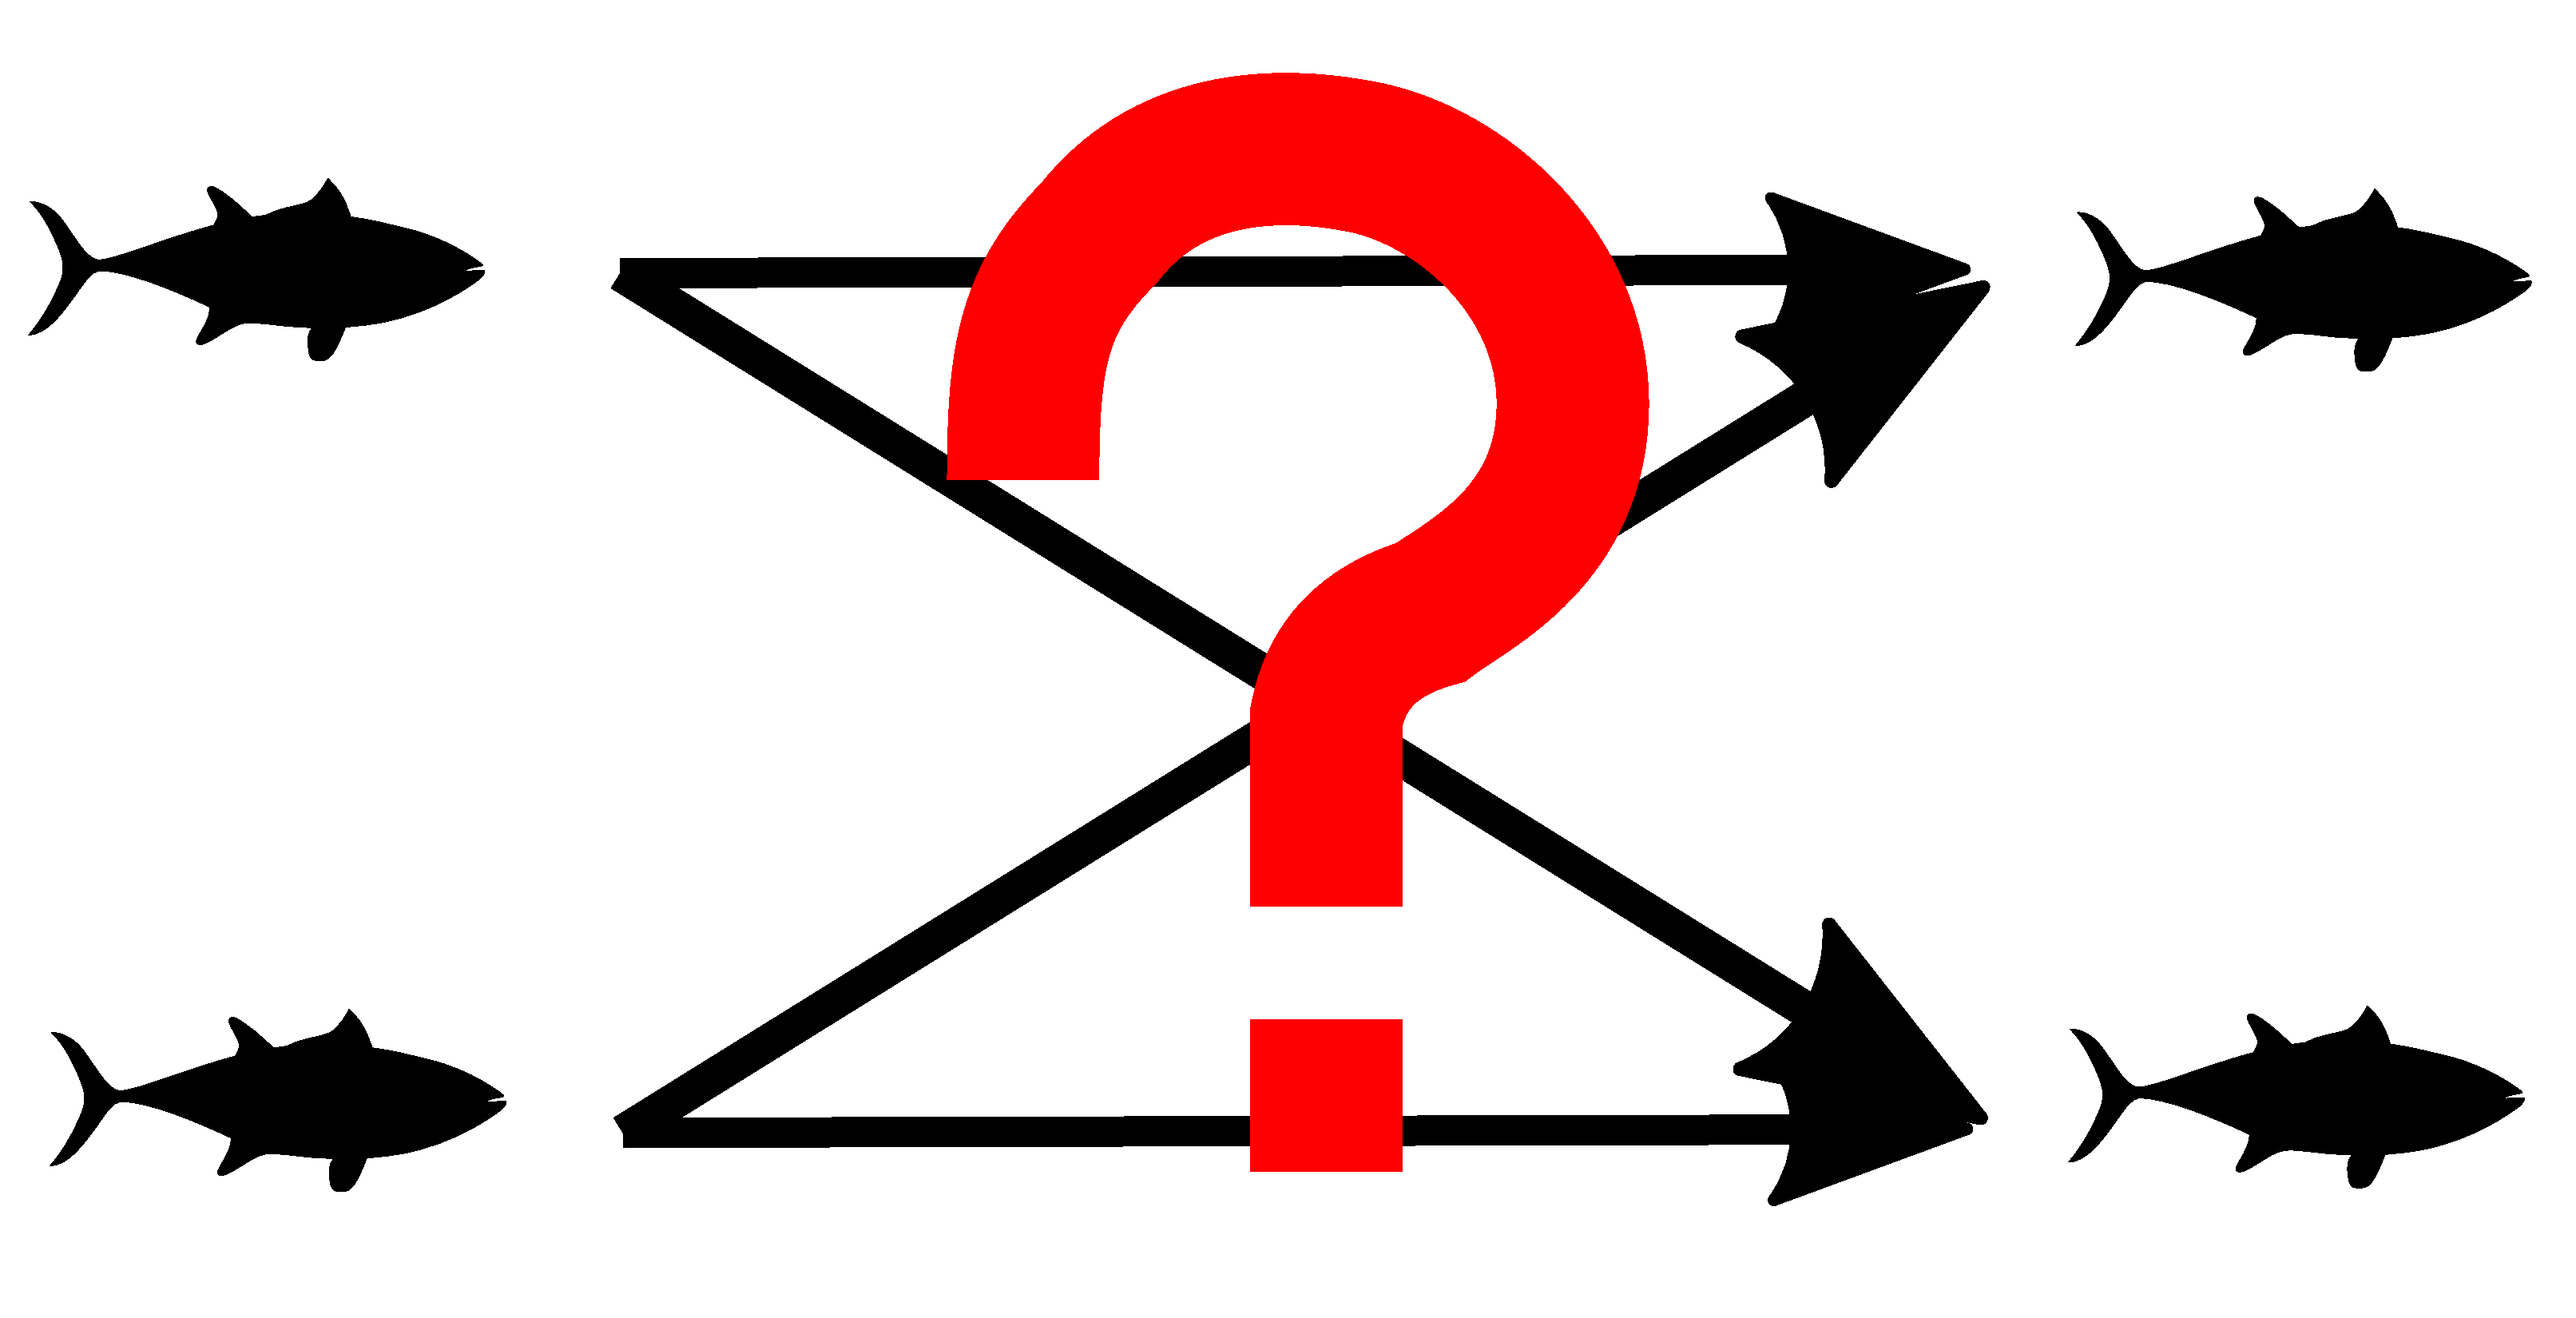
\includegraphics[width=.5\textwidth]{fish1}
	\caption{}
\end{figure}
\textbf{Figure 1} There are two methods of unswapping which we will deploy. The first is during frame groups(ranges) in which the software reports that there are two fishes, in which we will compare the distances between the fishes as if they were both swapped and unswapped, and compute which value is smaller.
\begin{figure}[h] 
	\centering
	\includegraphics[width=.5\textwidth]{fish2}
	\caption{}
\end{figure}
\textbf{Figure 2} If that doesn't work due to the software returning the output that there is only one fish due to the fish being in the same place and the software being unable to tell the fish apart, we look for an unique identifier for the fishes, which in this case is their average brightness. We then compare the similarity of the 2d histograms to determine the identity of the fish. \par

\section{Results}

\subsection{Data Structure}
The first operation performed was parsing the video and converting it to a [n,m,o,1] array, which has size of ``the number of frames'' by ``number of the fish'' by ``the number of pixels in each fish'', by ``a triplet consisting of the x coordinate of the fish, the y coordinate, and the greyscale rgb value in the form [x,y,g]''. 

\subsection{Identifying Nonoverlapping Ranges}

Since the primary method of unswapping does not work in frames in which there is only one fish returned, the first step is to find the frames in which the software is reading that there are two fish, so that we can only run the unswapping code on those frames. We do this by running through every frame and returning the ones that fit our criteria in a list that we can then reference.

\begin{minipage}[c]{\textwidth}
\begin{lstlisting}[language=Python]
i2=0
nonOverlappingRange=[]
while i2<len(fish):
    i1=i2
    while i1<len(fish) and len(fish[i1])!=2:
        i1+=1
    i2=i1
    while i2 < len(fish) and len(fish[i2])==2:
        #find the first overlapping index
        i2+=1
    nonOverlappingRange.append([i1,i2])
print(nonOverlappingRange)
\end{lstlisting}
\end{minipage}

We then take the data and find the center of each fish to allow us to perform analysis on a singular point instead of trying to perform analysis on the entirety of the fish, due to how much easier it is to compute distances in that method. 
\begin{figure}[h] 
	\centering
	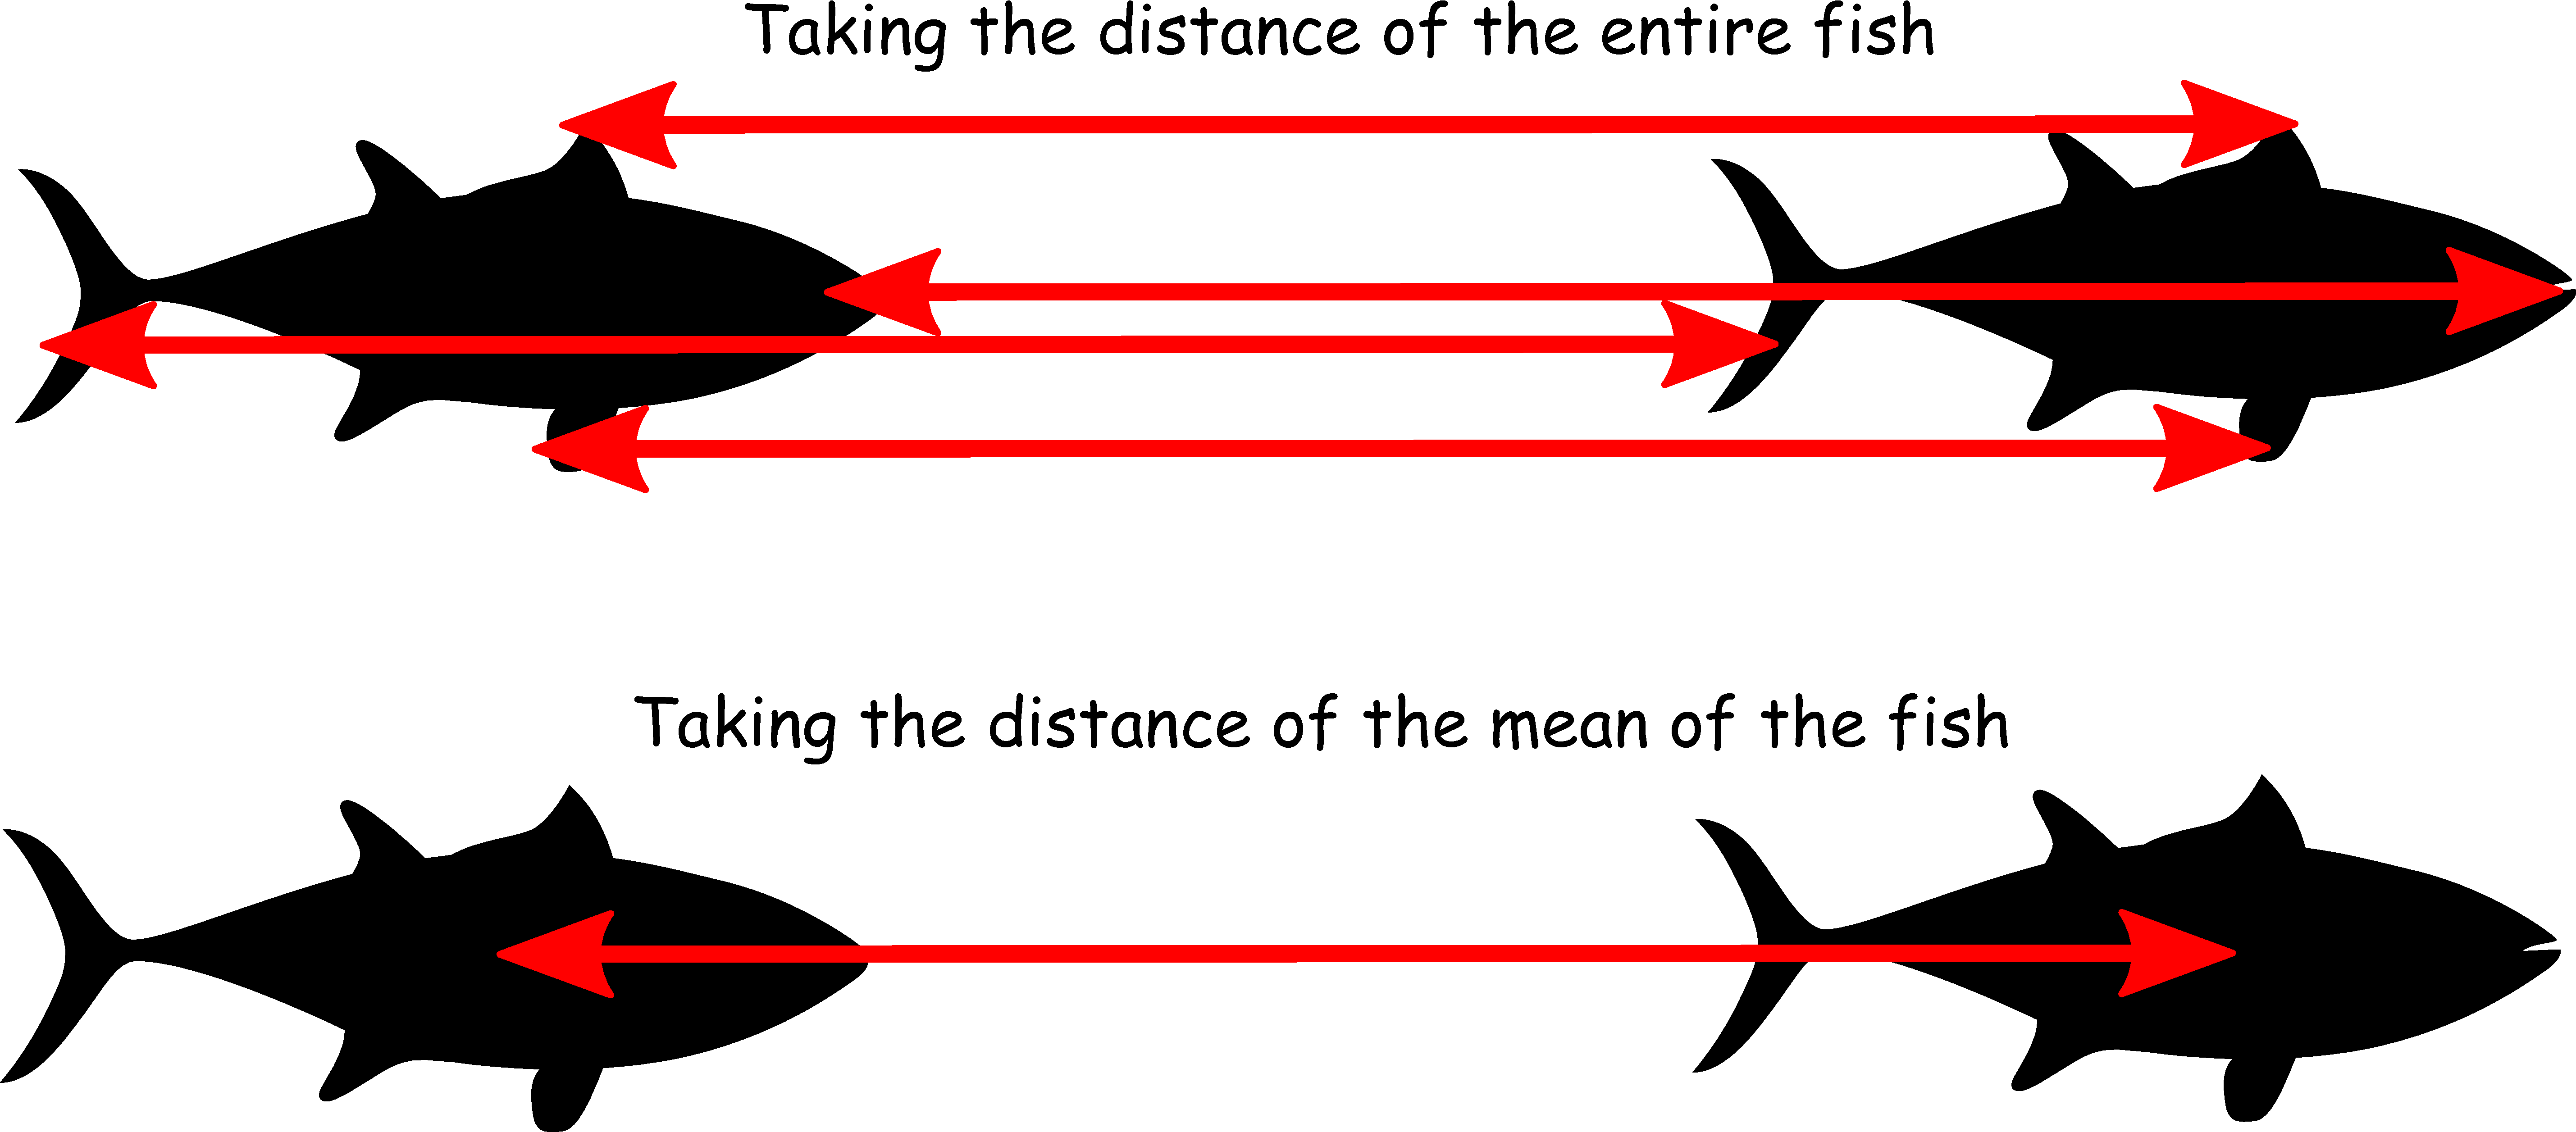
\includegraphics[width=.5\textwidth]{fish3}
	\caption{}
\end{figure}\textbf{Figure 3}

\begin{minipage}[c]{\textwidth}
\begin{lstlisting}[language=Python]
fishMean=[]
for i in range(len(fish)):
    if len(fish[i])==1:
        fishMean.append([[np.mean(fish[i][0].T[0]),np.mean(fish[i][0].T[1])],[np.mean(fish[i][0].T[0]),np.mean(fish[i][0].T[1])]])
    else:
        fishMean.append([[np.mean(fish[i][0].T[0]),np.mean(fish[i][0].T[1])],[np.mean(fish[i][1].T[0]),np.mean(fish[i][1].T[1])]])
fishMean=np.asarray(fishMean)
#fishMean[i.j.k] is the coordinate of k of the position of fish j in frame i
\end{lstlisting}
\end{minipage}

\subsection{Distance Based Unswapping}

Once we have the fish imported and then converted into a format that is easier to work with, we then can start to unswap the fish. However, we will be restricting ourselves to the nonoverlapping ranges, since comparing the fish frame-to-frame for unswapps is pointless when the software only returns one fish. The first step to unswapping the fishes is to calculate which frames are swapped by comparing the distances between the two fishes at each consecutive frame pair as if they were both cases and returning the lesser of the two distances as the one that is the correct fish continuity. To do this, we offload most of the actual calculation to a function that puts the 4 possible distances into a matrix and uses numpy's linalg.norm to compare the iterations.

\begin{minipage}[c]{\textwidth}
\begin{lstlisting}[language=Python]
def swapStatus(pos,i):
    '''
    Detect swaps between consecutive frames based on proximity.
    
    Input:
        pos: Positions. Array with shape (Nframes,Nfish,Ndimensions),
        i: Frame index. Int.
    
    Output:
        Int. 0 if no swaps, 1 if swapped, 2 if overlapping.
    '''
    nFish=pos.shape[1] #Number of fish
    distanceMatrix=[np.linalg.norm(pos[i+1][0]-pos[i][0]),
                    np.linalg.norm(pos[i+1][1]-pos[i][1]),
                    np.linalg.norm(pos[i+1][0]-pos[i][1]),
                    np.linalg.norm(pos[i+1][1]-pos[i][0])]
    swapCriteron=(distanceMatrix[0]+distanceMatrix[1])-(distanceMatrix[2]+distanceMatrix[3])
    if abs(swapCriteron)<1e-10:
        return 2 #Overlapping
    elif swapCriteron>0:
        return 1 #Swapped
    elif swapCriteron<0:
        return 0 #Normal
    else:
        return -1
\end{lstlisting}
\end{minipage}

This function returns a value of  either 0(Maintaining continuity), 1(Swapped), or 2(Overlapping region) that we then can reference later.

We then can call on the function to return a list of the swap status of the fishes.

\begin{minipage}[c]{\textwidth}
\begin{lstlisting}[language=Python]
statusList=[]
for i in range(len(fishMean)-1):
    statusList.append(swapStatus(fishMean,i))
print(collections.Counter(statusList))
\end{lstlisting}
\end{minipage}

This then allows us to start unswapping the fish. To do this we first have to find the start and end points for the swap, since if we were to unswap at every point we would just reduce the number of swaps by one. However, we do get to say that every other unswap is a terminus, at least within nonoverlapping ranges, for the sake of simplicity. The next step is to structure the data in a format that allows for unswapping. The format that is easiest for us to work with (in this case) is an array of the indexes of the frames where the overlapping occurs, which we then can use by applying a swapping rule to fishMean directly.

\begin{minipage}[c]{\textwidth}
\begin{lstlisting}[language=Python]
posU=fishMean.copy()
for j,i in I:
    posU[j:i,:]=pos[j:i,[1,0]]
\end{lstlisting}
\end{minipage}

At this point, all the data inside the nonoverlapping regions has been unswapped, and a simple check with collections.Counter reveals that we have been successful in that regard.

\begin{minipage}[c]{\textwidth}
\begin{lstlisting}[language=Python]
status=[]
for i in range(len(posU)-1):
    status.append(swapStatus(posU,i))
print(collections.Counter(status))
\end{lstlisting}
\end{minipage}
\begin{verbatim}
Counter({0: 49283, 2: 1930})
\end{verbatim}

\subsection{Texture-based Unswapping}
The next step of this process is to find the frame segments in which the program swaps the fish during the overlapping regions. To do this we must construct 2d histograms of the sum and difference of brightness values for each fish during each nonoverlapping range, which we then can take the on and off axis distance of to determine swaps.

%\textbf{Include 2d histograms?}

\section{Conclusion}

The end result of the current state of this project is that we have a program that can take the input of a video of fishes, and return the positions of each fish at each frame correctly, at least for two fish. This is a starting point for any and all analysis that can be performed on the fishes, including schooling and predictive behaviour analysis. The next steps for this project include writing the code that unswapps over overlapping ranges, and eventually scaling the project to more than 2 fishes.

\end{document}
